\section{Jackknife Analysis}

In this problem, we will see how the jackknife method can be used to find errors on functions
on the mean values of data, i.e., on \(f(\bar{v}_a)\).
We can use the universe of data to calculate
the errors and then calculate the same error from a sample of size \(N = 5000\).

We will consider two functions in what follows
%
\begin{align}
    f_1(\bar{v}_1, \bar{v}_2) & = \frac{ \bar{v}_1 }{ \bar{v}_2 }, \\
    f_2(\bar{v}_3, \bar{v}_4) & = \exp( \bar{v}_3 - \bar{v}_4 ).
\end{align}

\Question{p2q1} Break the \(M\) measurements up into groups of size \(N\), calculate
\(\bar{v}_a\) for each group and then calculate \(f_i(\bar{v}_a)\) for each group.
Calculate these functions of the data means for all \(M/N\) groups and find the
standard deviation for \(f_i(\bar{v}_a)\), i.e., \(\hat{\sigma}_{f_i,N}\).

\Answer{}
For \(N = 5000\), there are \(320\) samples for each variable.
The sample means for each variable are shown in Figure~\ref{fig:sample_means}.
We can see that these data, at least over the range of \(5000\) numbers,
show similar trends.
It could suggest that these \(5\) variables are generated using the same random
number generator.

\begin{figure}[h]
    \centering
    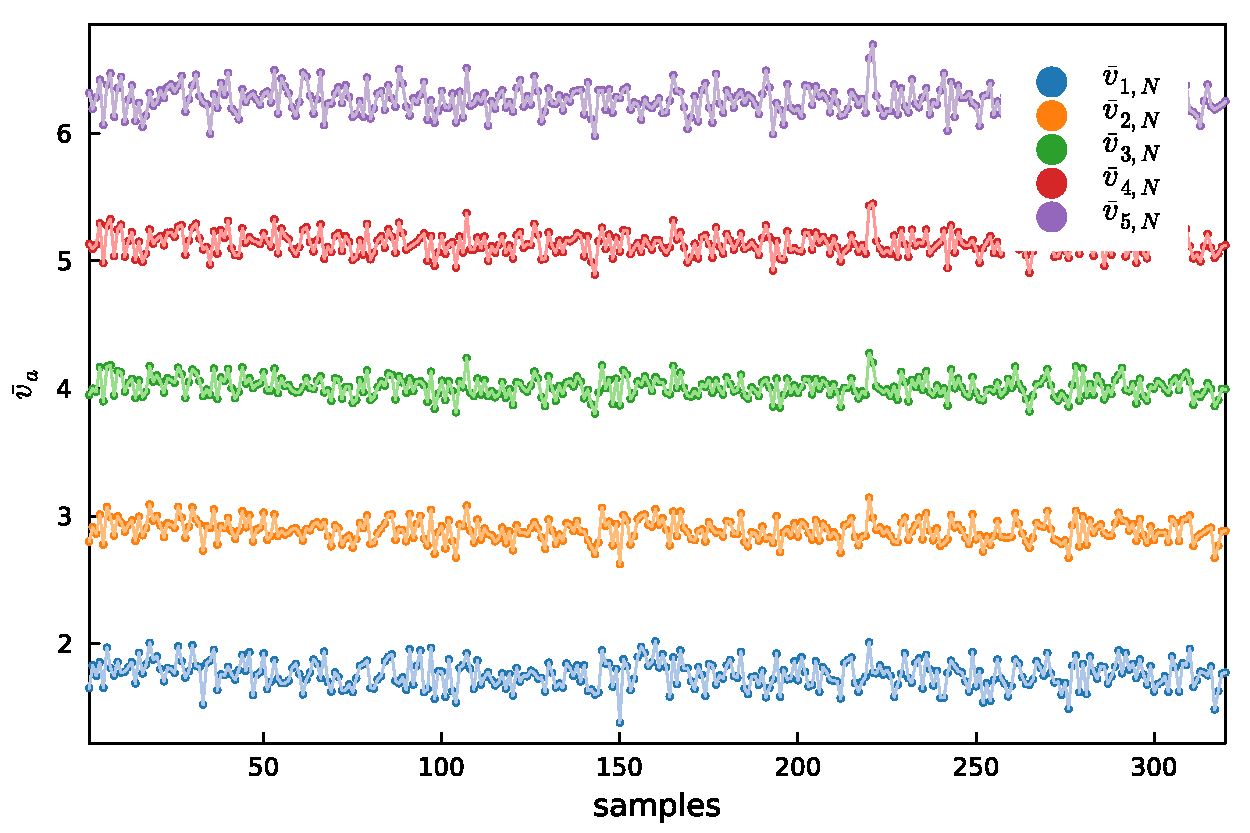
\includegraphics[width=0.8\textwidth]{sample_means}
    \caption{The sample means \(\bar{v}_a\) for variables \(v_a\), where
        \(a = 1\), \(\ldots\), \(5\) when \(N = 5000\).}
    \label{fig:sample_means}
\end{figure}

We plot \(f_1(\bar{v}_1, \bar{v}_2)\) and \(f_2(\bar{v}_3, \bar{v}_4)\) in
Figure~\ref{fig:fi}.

Since \(f_1\) and \(f_2\) can only be applied to the average values such as
\((\bar{v}_{1,\eta}, \bar{v}_{2,\eta})\) and \((\bar{v}_{3,\eta}, \bar{v}_{4,\eta})\)
for \(\eta = 1\), \(\ldots\), \(320\), we need to adapt Equation~\eqref{eq:varva}
to the following form:
%
\begin{equation}
    \hat{\mathbb{V}}(f_1) = \frac{ 1 }{ M / N - 1 }
    \sum_{\eta=1}^{M/N} \bigl( \bar{f}_{1,\eta} - \barhat{f}_1 \bigr)^2
\end{equation}
%
where we denote \(\bar{f}_{1,\eta} = f_1(\bar{v}_{1,\eta}, \bar{v}_{2,\eta})\),
and
%
\begin{equation}
    \barhat{f}_1 = \frac{ N }{ M } \sum_{\eta=1}^{M/N} \bar{f}_{1,\eta}
\end{equation}
as the true mean of \(f_1\)
since \(f_1(\bar{v}_{1,\eta}, \bar{v}_{2,\eta})\) is already a function of the means.
Therefore, the true standard deviation \(\hat{\sigma}_{f_i,N}\) is
%
\begin{equation}
    \hat{\sigma}_{f_i,N} = \sqrt{\hat{\mathbb{V}}(f_1)}.
\end{equation}

\begin{figure}
    \centering
    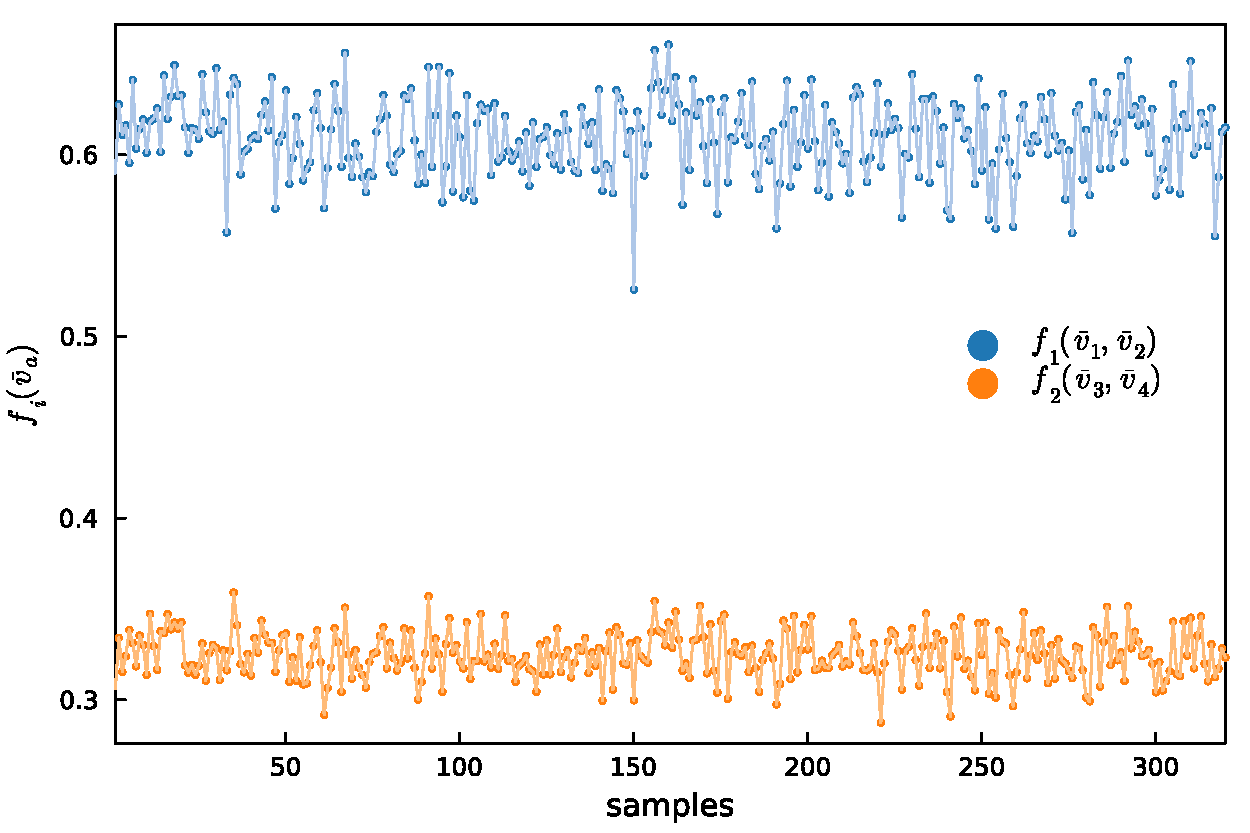
\includegraphics[width=0.8\textwidth]{f1_f2}
    \caption{Plot \(f_1(\bar{v}_1, \bar{v}_2)\) and \(f_2(\bar{v}_3, \bar{v}_4)\) for each group of variable pairs.}
    \label{fig:fi}
\end{figure}

As discussed, the mean and standard deviation of \(f_1\) and
\(f_2\) are listed in Table~\ref{tab:stdf1f2}.

\begin{table}
    \centering
    \caption{The mean and standard deviation of \(f_1\) and \(f_2\) from all \(M\) values.}
    \label{tab:stdf1f2}
    \begin{tabular}{@{}cccc@{}}
        \toprule
        \(\barhat{f}_1\) & \(\barhat{f}_2\) & \(\hat{\sigma}_{f_1,N}\) & \(\hat{\sigma}_{f_2,N}\) \\
        \midrule
        \(0.60956\)      & \(0.32481\)      & \(0.0214303\)            & \(0.0126915\)            \\
        \bottomrule
    \end{tabular}
\end{table}


\Question{} Calculate \(\hat{\sigma}_{f_i,N}\) from naïve propagation of errors, i.e., using
\(\hat{\sigma}_{\bar{v}_a,N}\) and neglecting correlations between the \(v_i\). Compare with
your results from Question~\ref{p2q1}.

\Answer{}
If we Taylor expand \(\hat{\Var}(f(\bar{x}, \bar{y}))\) up to the first order, we will
get
%
\begin{equation}\label{eq:varf}
    \hat{\Var}(f(\bar{x}, \bar{y})) =
    \biggl(\frac{ \partial f }{ \partial x } \at{x = \barhat{x}}\biggr)^2 \hat{\Var}(\bar{x}) +
    \biggl(\frac{ \partial f }{ \partial y } \at{y = \barhat{y}}\biggr)^2 \hat{\Var}(\bar{y}) +
    2\biggl(\frac{ \partial f }{ \partial x } \at{x = \barhat{x}}\biggr)
    \biggl(\frac{ \partial f }{ \partial y } \at{y = \barhat{y}}\biggr)
    \hat{\sigma}(\bar{x}, \bar{y}).
\end{equation}
%
But since we are considering naïve propagation of errors, i.e.,
%
\begin{equation}
    \hat{\sigma}(\bar{x}, \bar{y}) \approx 0,
\end{equation}
%
then~\eqref{eq:varf} will be reduced to
%
\begin{equation}\label{eq:reducedvarf}
    \hat{\Var}(f(\bar{x}, \bar{y})) =
    \biggl(\frac{ \partial f }{ \partial x } \at{x = \barhat{x}}\biggr)^2 \hat{\Var}(\bar{x}) +
    \biggl(\frac{ \partial f }{ \partial y } \at{y = \barhat{y}}\biggr)^2 \hat{\Var}(\bar{y}).
\end{equation}
%
Therefore, the variance of \(f_1\) and \(f_2\) are:
%
\begin{align}
    \hat{\Var}(f_1(\bar{v}_1, \bar{v}_2)) & =
    \frac{ 1 }{ \barhat{v}^2_2 } \hat{\Var}(\bar{v}_1) +
    \frac{ \barhat{v}^2_1 }{ \barhat{v}^4_2 } \hat{\Var}(\bar{v}_2) =
    \biggl(\frac{ 1 }{ \barhat{v}_2 } \sgbar{1}\biggr)^2 +
    \biggl(\frac{ \barhat{v}_1 }{ \barhat{v}^2_2 } \sgbar{2} \biggr)^2, \\
    \hat{\Var}(f_2(\bar{v}_3, \bar{v}_4)) & =
    \exp( \barhat{v}_3 - \barhat{v}_4 )^2 \bigl(\hat{\Var}(\bar{v}_3) + \hat{\Var}(\bar{v}_4)\bigr) =
    \exp( \barhat{v}_3 - \barhat{v}_4 )^2 \bigl(\sgbar{3}^2 + \sgbar{4}^2\bigr),
\end{align}
%
where we calculate \(\sgbar{a}\) the same way as we have done in \label{p1q2}.

Hence, the estimated standard deviation of \(f_1\) and \(f_2\) are
\(\hat{\sigma}_{f_1,N} = 0.0415114\) and \(\hat{\sigma}_{f_2,N} = 0.0392291\).
As we can see, these values are quite far from the ones we obtained in
Table~\ref{tab:stdf1f2}.
We could conclude that~\eqref{eq:reducedvarf} is a rather lousy approximation.


\Question{} We now want to estimate \(\sigma_{\bar{v}_a,N}\) and \(\sigma_{f_i,N}\) using
the jackknife method from a single sample of size \(N\).
First, we must deal with the autocorrelations in the data, and you have an idea of the
integrated autocorrelation time from the first problem. We proceed as follows here. Average
your \(N\) data values into bins of size \(b\). This will produce \(N/b\) data values.
Then use the jackknife method to estimate \(\bar{v}_a\) and \(\sigma_{\bar{v}_a,N}\) from
these \(N/b\) data values. The jackknife method resums these \(N/b\) values as done in class,
i.e.,
%
\begin{equation}
    v'_{a,k} = \frac{ 1 }{ N / b - 1 } \sum_{i=1, i \neq k}^{N/b} v_{a,i}.
\end{equation}

From these jackknife values, you can determine \(\bar{v}_a\) and \(\sigma_{\bar{v}_a,N}\).
Do this for a few different values of \(b\) comparable to the integrated autocorrelation
time to check that your results do not depend strongly on \(b\).

\Answer{}
In the following text, we select the first \(5000\) values of each variable as our original
samples of data.

To estimate the population mean of variable \(x\),
the natural estimator is the sample mean
%
\begin{equation}
    \bar{x} = \frac{ 1 }{ N } \sum_{i=1}^N x_i.
\end{equation}
%
The definition of jackknife resampling is
%
\begin{equation}
    x_k' = \frac{1}{N - 1}
    \sum_{i \neq k} x_i = \frac{ 1 }{ N - 1 } \Bigl(\sum_i x_i - x_k \Bigr),
\end{equation}
%
where \(k = 1\), \(\ldots\), \(N\), and \(x'_k\) is called the \(k\)-th jackknife replicate.
The algorithm is shown in Snippet~\ref{lst:jackknife}.
%
\begin{algorithm}
    \caption{The jackknife resampling algorithm written in Julia.}
    \label{lst:jackknife}
    \begin{juliacode}
        struct JackknifeSampler <: Sampler end

        function sampleby(sample::Sample, ::JackknifeSampler)
            f = inv(length(sample) - 1)
            return Sample(f * map(eachindex(sample)) do j
                sum(sample[filter(≠(j), eachindex(sample))])
            end)
        end
    \end{juliacode}
\end{algorithm}

After dividing the data of size \(N\) into \(N/b\) groups, we then do a jackknife resampling.
For \(\bar{x}\), the mean of the jackknife data and the original data should be the
same, i.e.,
%
\begin{equation}
    \frac{ 1 }{ N } \sum_k x_k' = \bar{x} = \frac{ 1 }{ N } \sum_k x_k.
\end{equation}
%
The means of these \(N/b\) groups of data with each group as an average of \(b\) original
values, are plotted in Figure~\ref{fig:JA_sample_means:a}.
As we can see, these \(\bar{v}_a\) are almost constants for different sizes of bins \(b\),
with very few variations.
That is, the estimated \(\bar{v}_a\) do not strongly depend on \(b\).
To have a clearer view of how these data changes, we plot \(\bar{v}_a - \barhat{v}_a\)
as a function of \(b\), where the ``true mean'' \(\barhat{v}_a\) is the mean of
the means, as shown in Figure~\ref{fig:JA_sample_means:b}.
Here, to minimize the grouping bias, we select all \(b\) to be factors of \(5000\),
so that there is only an integer number of groups.

\begin{figure}
    \centering
    \begin{minipage}[t]{0.8\linewidth}
        \centering
        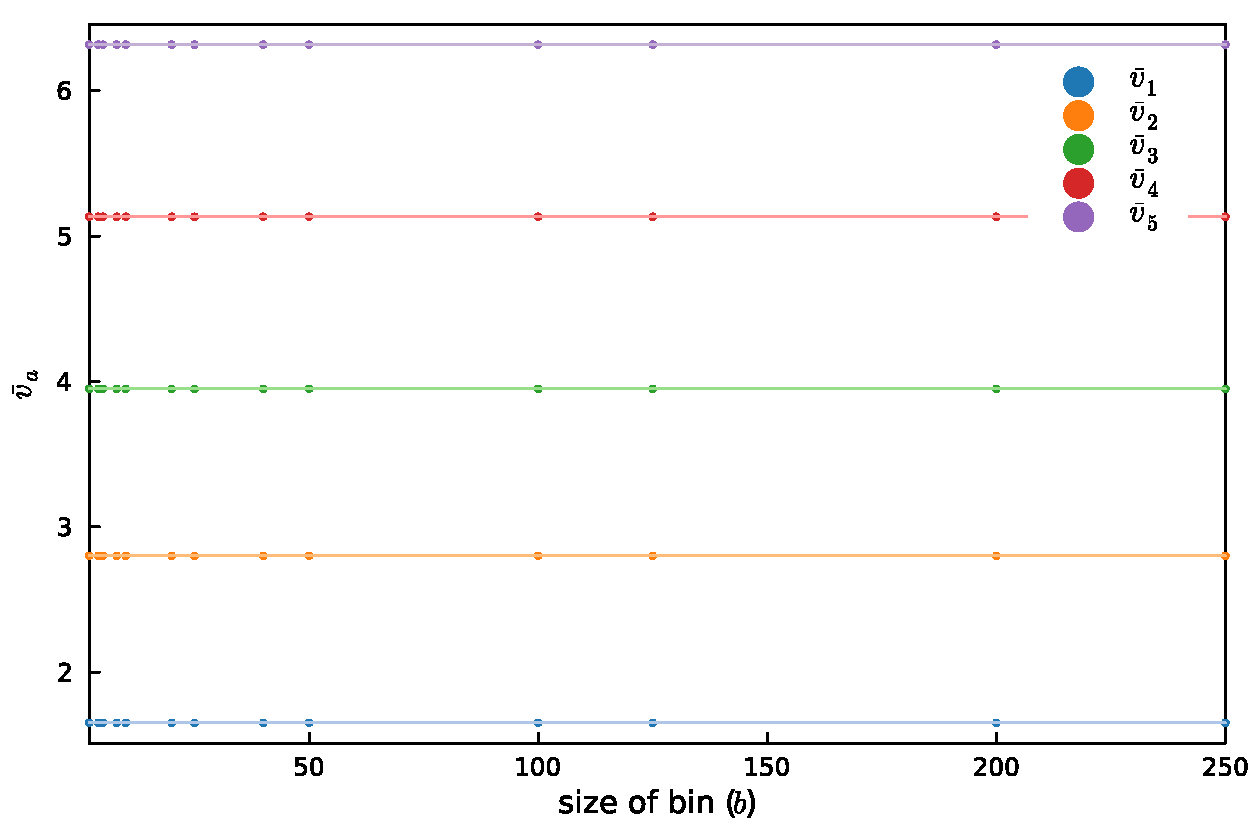
\includegraphics[width=\linewidth]{JA_sample_means}
        \subcaption{The average values of these \(N/b\) groups as a function of
            sizes of bins \(b\).}
        \label{fig:JA_sample_means:a}
    \end{minipage}
    \hfill
    \begin{minipage}[t]{0.8\linewidth}
        \centering
        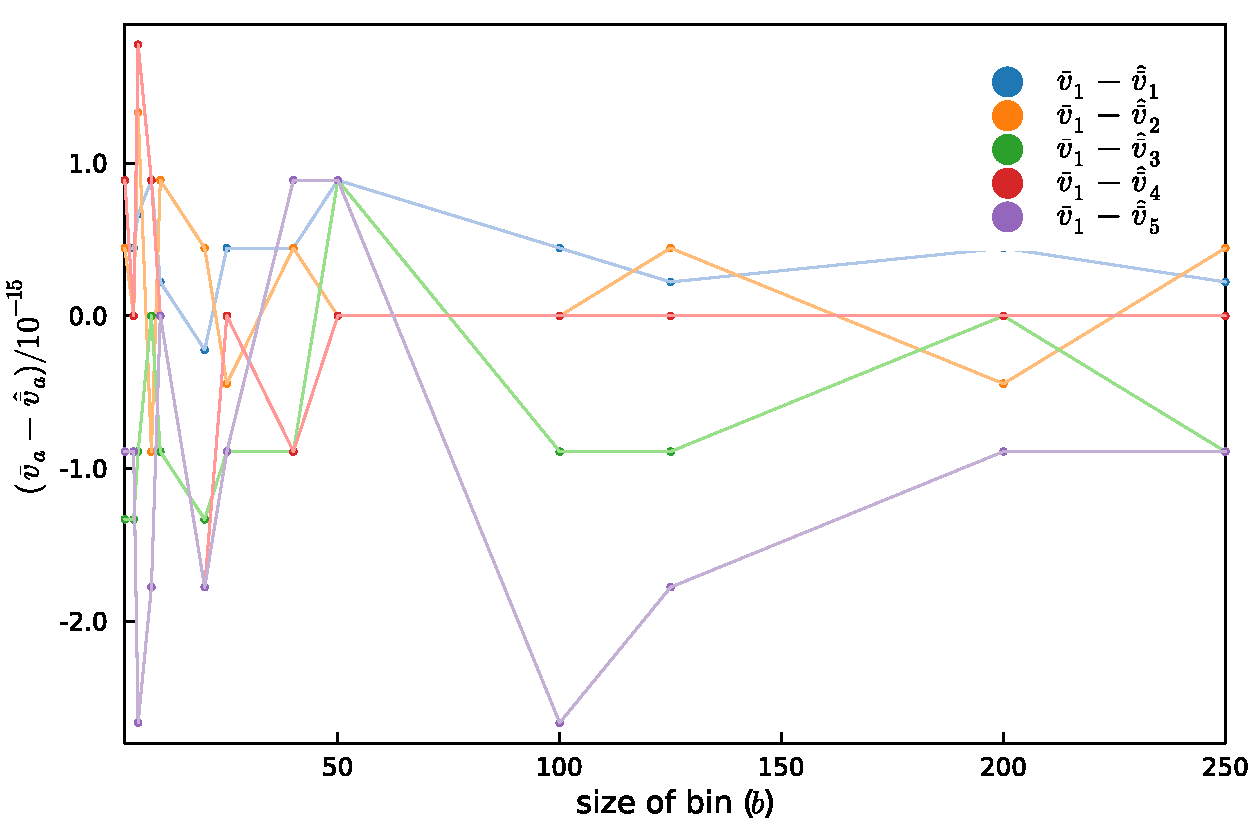
\includegraphics[width=\linewidth]{JA_sample_deviations}
        \subcaption{The average values subtracted by the true mean of these \(N/b\) groups as
            a function of sizes of bins \(b\), with \(y\)-axis scaled by a factor of
            \(10^{15}\).}
        \label{fig:JA_sample_means:b}
    \end{minipage}
    \caption{The average values \(\bar{v}_a\) of the jackknife data as a function of \(b\).}
    \label{fig:JA_sample_means}
\end{figure}

\begin{figure}
    \centering
    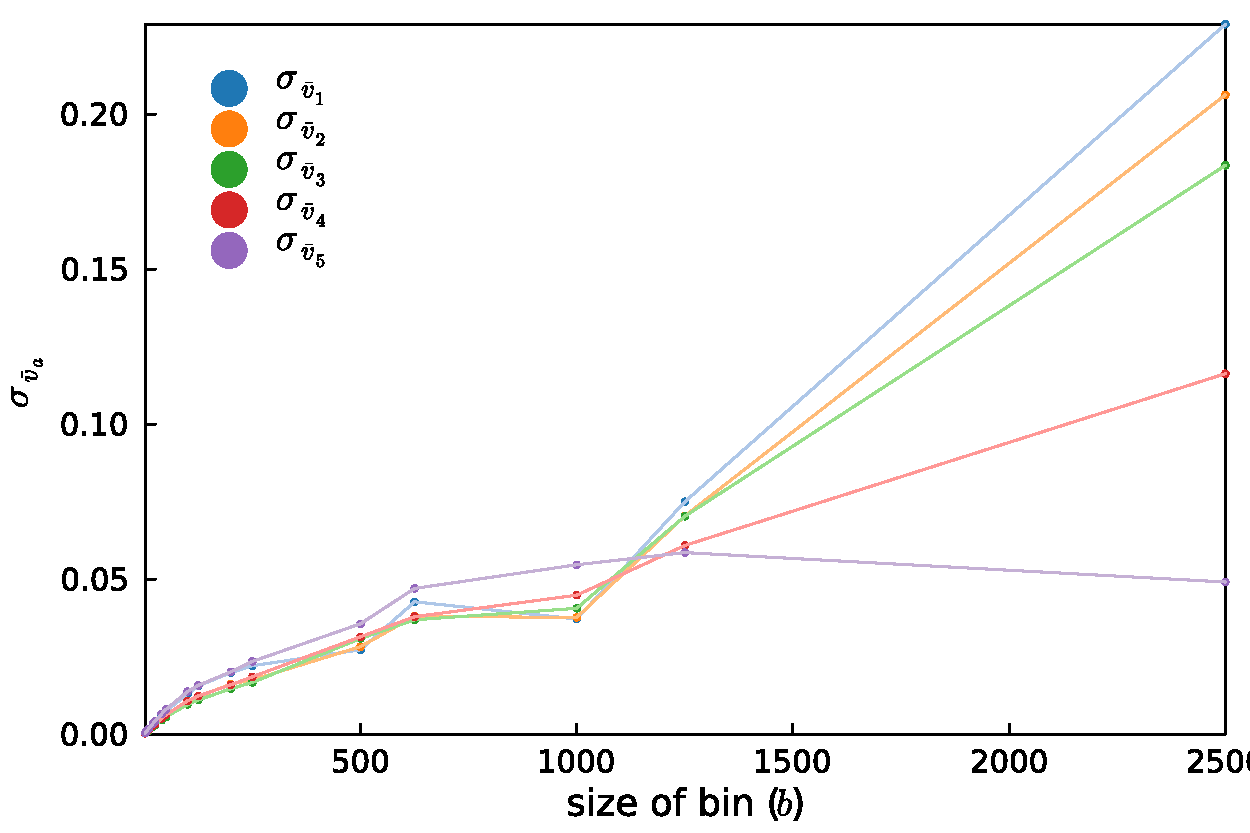
\includegraphics[width=0.8\textwidth]{JA_sample_std_wrong}
    \caption{Wrong standard deviation of the jackknife data (\(\sigma_{\bar{v}_a,N}\)) as a
        function of \(b\) since we did not put the correct factors in
        Equation~\eqref{eq:JAstd}.}
    \label{fig:JA_sample_std_wrong}
\end{figure}

A jackknife estimate of the variance of \(\bar{x}\) can be calculated from the variance of
the jackknife replicates:
%
\begin{equation}\label{eq:JAstd}
    \Var(x') = \frac{ N - 1 }{ N } \sum_k (x_k' - \bar{x})^2
    = \frac{ 1 }{ N (N - 1) } \sum_k (x_k - \bar{x})^2,
\end{equation}
%
where \(x'_k\) denotes the \(k\)-th jackknife replicate and \(x_k\) denotes the \(k\)-th
original value.
Note the correction factors \(\frac{ N - 1 }{ N }\) and \(\frac{ 1 }{ N (N - 1) }\),
you cannot omit them when doing such calculations. For example, if we treat
jackknife data as normal \code{Sample} types, which uses the normal variance relation:
%
\begin{equation}
    \Var(x) = \frac{ 1 }{ N - 1 } \sum_k (x_k - \bar{x})^2,
\end{equation}
%
then wrong results will be given, as shown in Figure~\ref{fig:JA_sample_std_wrong}.
This is because for bins of size \(b=2500\), for instance, there are only \(2\)
bins, and \(\frac{ 1 }{ N - 1 }\) will be larger than those when \(b\) are smaller.

Therefore, we need to define type \code{JackknifeSample} and fix the corresponding
\code{sampleby} method which we defined in Snippet~\ref{lst:jackknife} to let it return
a collection of \code{JackknifeSample}s,
as shown in Snippet~\ref{lst:newjackknife}.
%
\begin{algorithm}
    \caption{Define type \code{JackknifeSample} and fix the corresponding
        \code{sampleby} method.}
    \label{lst:newjackknife}
    \begin{juliacode}
        struct JackknifeSample{T} <: Data{T}
            data::Vector{T}
        end

        function sampleby(sample::Sample, ::JackknifeSampler)
            f = inv(length(sample) - 1)
            ∑ = sum(sample)
            return JackknifeSample([(∑ - value) for value in sample]) * f
        end
    \end{juliacode}
\end{algorithm}
%
We also need to redefine a new \code{var} method for \code{JackknifeSample}s,
as shown in Snippet~\ref{lst:varjackknife}.
%
\begin{algorithm}
    \caption{Calculate the variance of jackknife data using the correct formula.}
    \label{lst:varjackknife}
    \begin{juliacode}
        function var(sample::JackknifeSample)
            N, μ = length(sample), mean(sample)
            return (N - 1) / N * sum(abs2, sample .- μ)
        end
    \end{juliacode}
\end{algorithm}

After putting the correct factors before the squared terms, we will get
Figure~\ref{fig:JA_sample_std}.
As we can see, the standard deviation versus \(b\) varies much less than
Figure~\ref{fig:JA_sample_std_wrong}, except for \(b = 2500\), we still get very large
variation. But it is understandable since \(N/b = 2\) now, and \((N - 1) / N = 1/2\).
%
\begin{figure}[H]
    \centering
    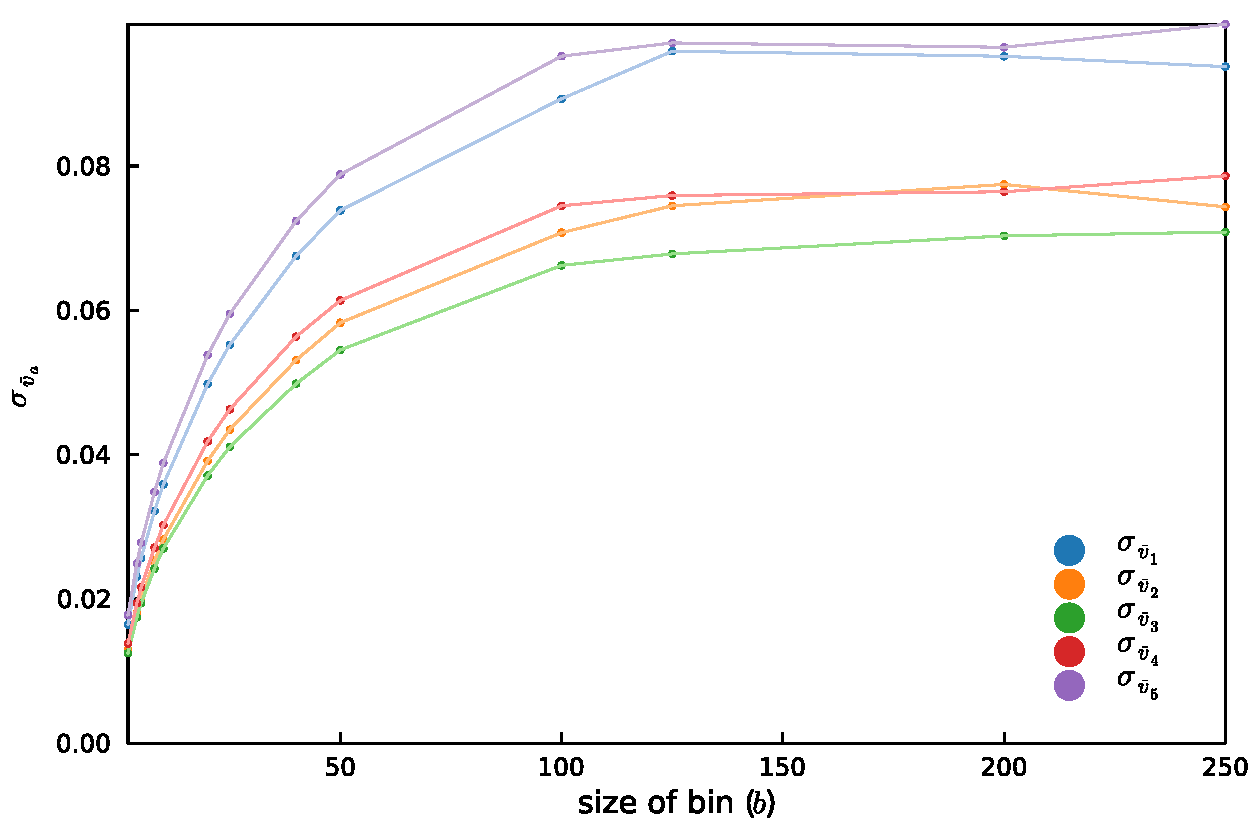
\includegraphics[width=0.8\textwidth]{JA_sample_std}
    \caption{The correct standard deviation of the jackknife data (\(\sigma_{\bar{v}_a,N}\)) as a
        function of \(b\).}
    \label{fig:JA_sample_std}
\end{figure}


\Question{} Now calculate \(f_i(v'_{a,k})\) for each of the \(N/b\) jackknife blocks.
You can then determine \(\sigma_{f_i,N}\) from
%
\begin{equation}\label{eq:sigmaf}
    \sigma^2_{f_i,N} = \frac{ N/b - 1 }{ N/b }
    \sum_{k=1}^{N/b} \bigl( f_i(v'_{a,k}) - f_i(\bar{v}_a) \bigr)^2.
\end{equation}
%
Again, do this for a few values of \(b\) that are comparable to the integrated
autocorrelation time. How does \(\sigma_{f_i,N}\) compare with \(\hat{\sigma}_{f_i,N}\) from
Question~\ref{p2q1}?

\Answer{}
Expand Equation~\eqref{eq:sigmaf} as
%
\begin{align}
    \sigma^2_{f_1,N} & = \frac{ N/b - 1 }{ N/b }
    \sum_{k=1}^{N/b} \bigl( f_1(v'_{1,k}, v'_{2,k}) - f_1(\bar{v}_1, \bar{v}_2) \bigr)^2, \\
    \sigma^2_{f_2,N} & = \frac{ N/b - 1 }{ N/b }
    \sum_{k=1}^{N/b} \bigl( f_2(v'_{3,k}, v'_{4,k}) - f_2(\bar{v}_3, \bar{v}_4) \bigr)^2.
\end{align}
%
We plot \(\sigma^2_{f_1,N}\) and \(\sigma^2_{f_2,N}\) in Figure~\ref{fig:JA_f_std:a}
and Figure~\ref{fig:JA_f_std:b}.
As we can see, \(\sigma_{f_1,N}\) is around \(0.02\),
and \(\sigma_{f_2,N}\) is around \(0.0125\), which are close to the standard deviation
of \(f_1\) (\(\hat{\sigma}_{f_1,N} = 0.0214303\)) and
\(f_2\) (\(\hat{\sigma}_{f_2,N} = 0.0126915\))
from all \(M\) values listed in Table~\ref{tab:stdf1f2}.
%
\begin{figure}
    \centering
    \begin{minipage}[t]{0.8\linewidth}
        \centering
        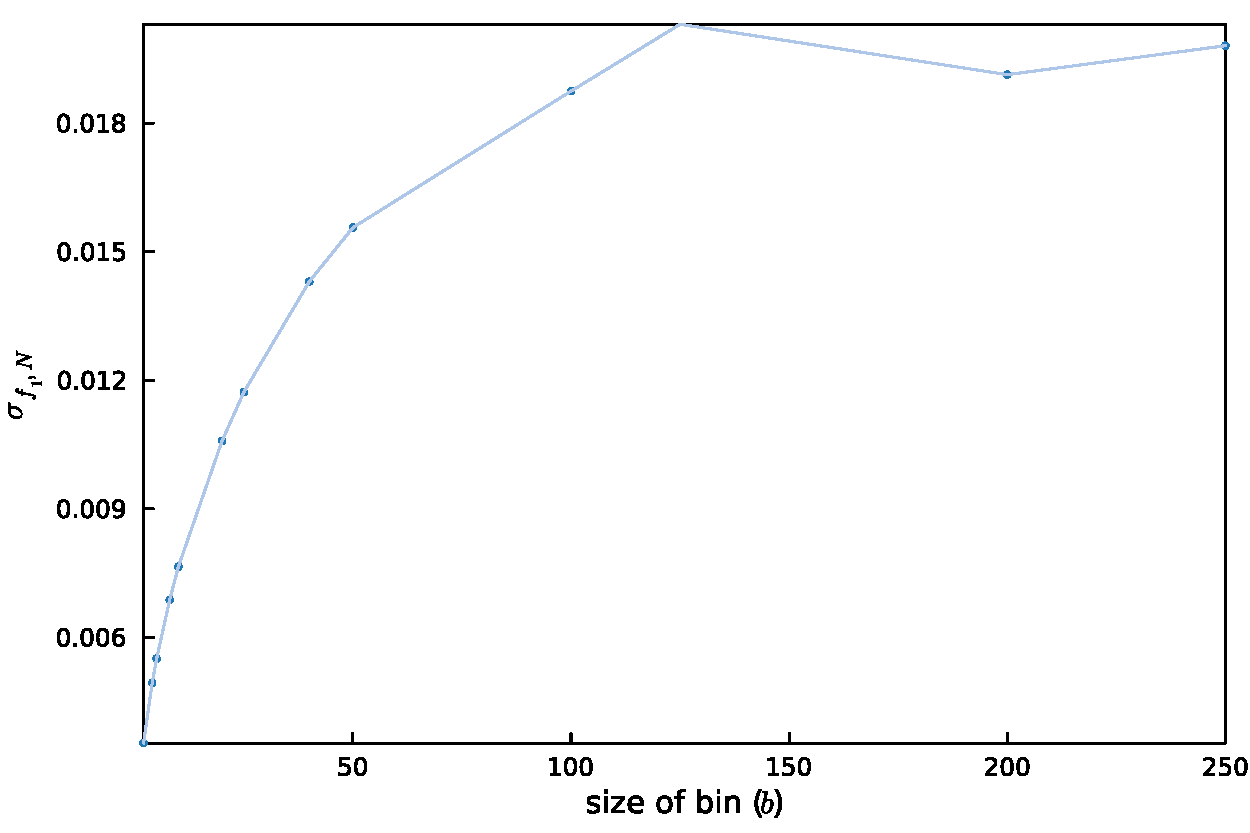
\includegraphics[width=\linewidth]{JA_f1_std}
        \subcaption{The standard deviation \(\sigma_{f_1,N}\) of these \(N/b\) groups as
            a function of sizes of bins \(b\).}
        \label{fig:JA_f_std:a}
    \end{minipage}
    \hfill
    \begin{minipage}[t]{0.8\linewidth}
        \centering
        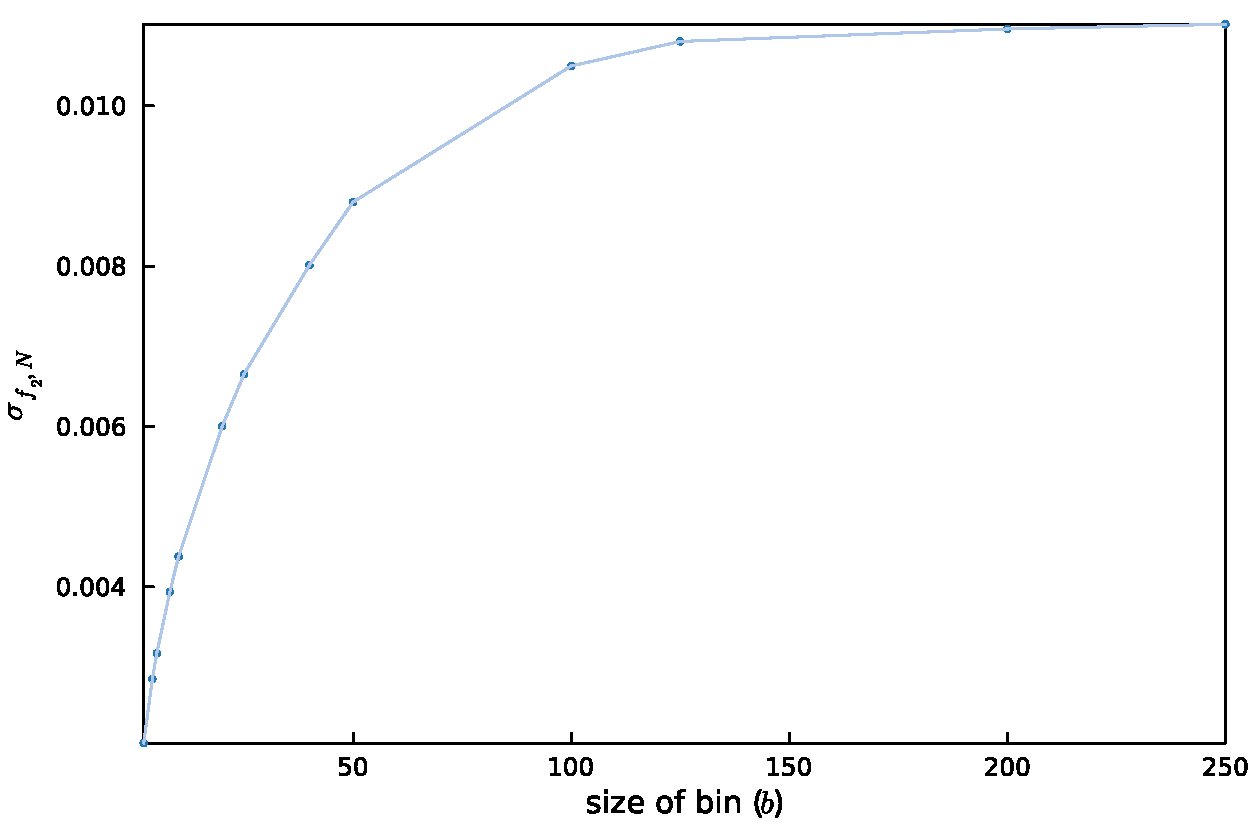
\includegraphics[width=\linewidth]{JA_f2_std}
        \subcaption{The standard deviation \(\sigma_{f_2,N}\) of these \(N/b\) groups as
            a function of sizes of bins \(b\).}
        \label{fig:JA_f_std:b}
    \end{minipage}
    \caption{Plot the standard deviations of \(f_1\) and \(f_2\) after jackknife resampling.}
    \label{fig:JA_f_std}
\end{figure}

Since we have the relation
%
\begin{equation}\label{eq:Deltaf}
    \frac{1}{N} \sum_{k=1}^N f(x'_k, y'_k) = f(\bar{x}, \bar{y}) +
    \mathcal{O}\Bigl(\frac{1}{N}\Bigr),
\end{equation}
%
where \(x'_k\) and \(y'_k\) are jackknife data.
We can verify this relation by plotting
%
\begin{equation}
    \Delta \bar{f} = \frac{1}{N} \sum_{k=1}^N f(x'_k, y'_k) - f(\bar{x}, \bar{y})
\end{equation}
%
for \(f_1\) and \(f_2\) respectively, as shown in Figure~\ref{fig:JA_f1_f2_mean}.
We can see from the figure that as the bin size \(b\) decreases, i.e., the number
of groups \(N / b\) increases, both \(\Delta \bar{f}_1\) and \(\Delta \bar{f}_2\)
converges to minimal values, as they should be (note the \(y\)-axis is of dimension
\(10^{-5}\)). That is, relation~\eqref{eq:Deltaf} holds.
%
\begin{figure}[H]
    \centering
    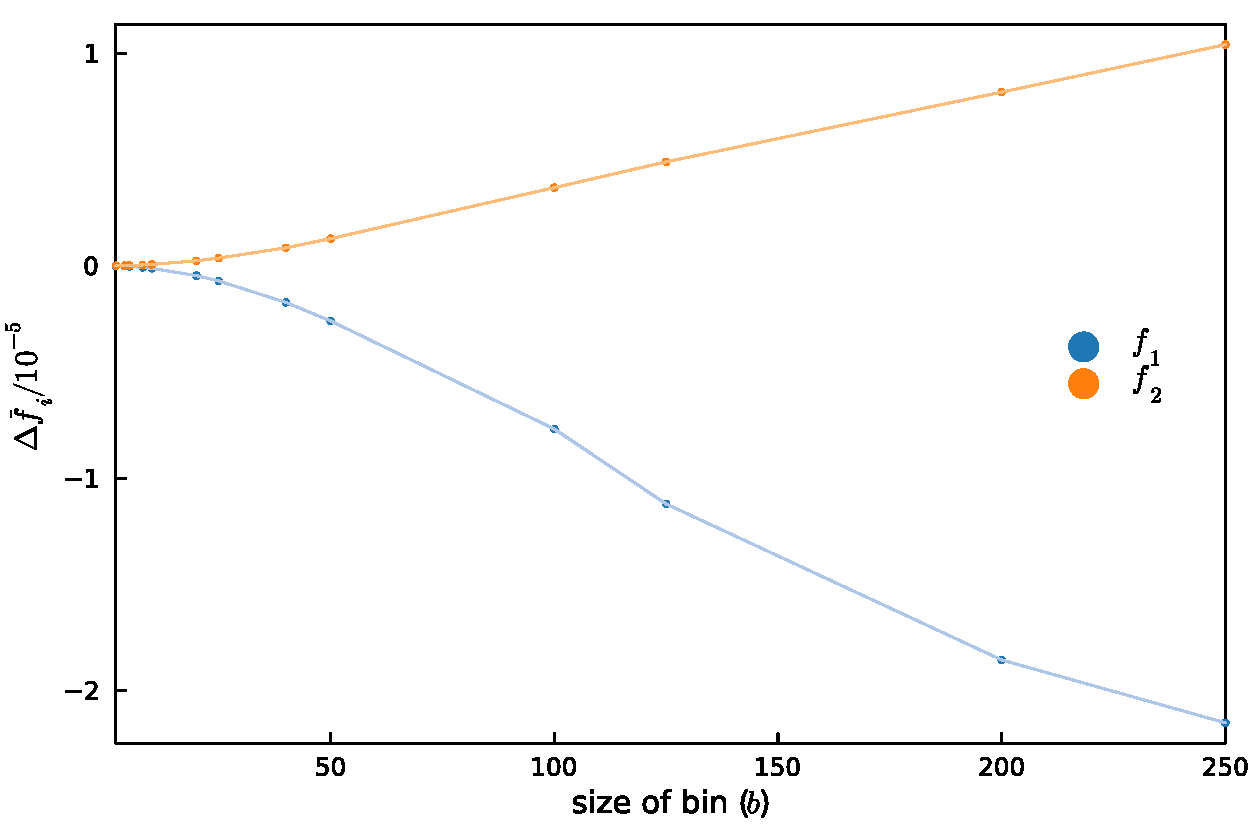
\includegraphics[width=0.8\textwidth]{JA_f1_f2_mean}
    \caption{The differences between \(\frac{1}{N} \sum_{k} f_i(v'_{a,k})\)
    and \(f_i(\bar{v}_a)\) for both \(f_1\) and \(f_2\) as a function of bin size
    \(b\), with \(y\)-axis scaled by a factor of \(10^5\).}
    \label{fig:JA_f1_f2_mean}
\end{figure}
